\documentclass[../main.tex]{subfiles}
\graphicspath{{\subfix{../images/}}}
\begin{document}
\section{Taylor series}
Taylor series enable us to approximate functions using polynomials. Polynomials are generally easier to manipulate so these can be extremely useful.

Using Taylor series we can approximate complicated functions at particular points with great accuracy.

The general form of a Taylor series about $x=a$ is:
\[p(x)=c_0 + c_1(x-a) + c_2(x-a)^2 + c_3(x-a)^3 + \dots\]

Or more specifically:
\[p(x)=\sum\limits_{n=0}^\infty c_n(x-a)^n\]

When we say "about \textit{a}" we mean that the approximation will be most accurate at that point as it is the centre of our approximating polynomial, and will get gradually less accurate the further away we get from \textit{a}.

\subsection*{Approximating $f(x)=\cos{(x)}$ with a quadratic}
To give an example, let's consider approximating the cosine function about zero with a quadratic.

\begin{figure}[h]
    \centering
    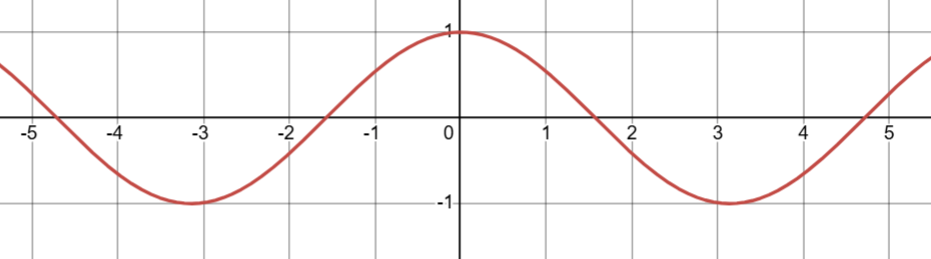
\includegraphics[width=0.5\textwidth]{images/taylorseries1.png}
\end{figure}

\textit{Note: a Taylor series about zero is also known as a Maclaurin series.}

Our general quadratic will be $p(x) = c_0 + c_1x + c_2x^2$.

To begin, we want our polynomial to be as accurate as possible at the point where $x=0$. So, we need to find the value of the cosine function when $x=0$. 

Since $f(0)=\cos{(0)}=1$, we can substitute this into our polynomial:
\[p(0) = 1 = c_0+c_1(0)+c_2(0)^2\]
\[\therefore c_0=1\]

Our polynomial is currently $p(x) = 1$, giving a great approximation at $x=0$ but terrible elsewhere.

\begin{figure}[h]
    \centering
    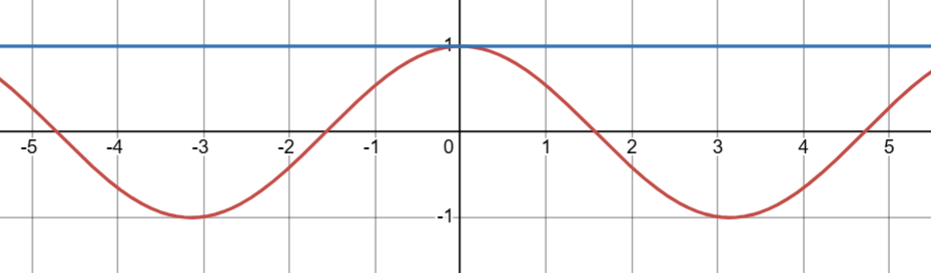
\includegraphics[width=0.5\textwidth]{images/taylorseries2.png}
\end{figure}

Next, we need to make sure that our approximating polynomial has the same gradient as cosine when $x=0$. We differentiate each function and substitute in $x=0$.

\[f'(x)=-\sin{(x)} \rightarrow f'(0)=0\]
\[p'(x)=c_1 + 2c_2x\]

Substituting in 0 for the gradient:
\[0=c_1 + 2c_2(0)\]
\[\therefore c_1=0\]

Our polynomial is currently $p(x) = 1 + c_2x^2$, still only giving a good approximation at $x=0$.

Finally, we have a quadratic so we want to make sure that the shape of the curve follows the same shape as the cosine graph as there are an infinite numnber of possible parabolas that could be applied. 

\begin{figure}[h]
    \centering
    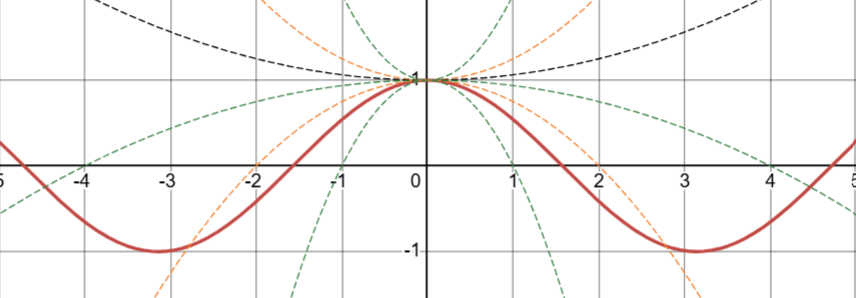
\includegraphics[width=0.5\textwidth]{images/taylorseries3a.png}
\end{figure}

At the point $x=0$ the cosine graph is concave down. To get the same shape we take the second derivatives:

\[f''(x)=-\cos{(x)} \rightarrow f''(0)=-\cos{(0)}=-1\]
\[p''(x)= 2c_2 \rightarrow 2c_2 = -1\]
\[c_2 = -\frac{1}{2}\]

Therefore, our polynomial is $p(x) = 1 - \frac{x^2}{2}$ 

You can see below that this gives a reasonable approximation for cosine near $x=0$, but starts to diverge around $\pm1$ radian.

\begin{figure}[h]
    \centering
    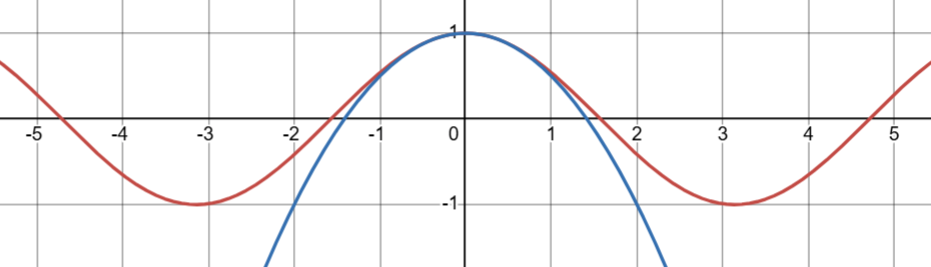
\includegraphics[width=0.5\textwidth]{images/taylorseries3.png}
\end{figure}

Remember, we derived a Taylor series about $x=0$ (also known as a Maclaurin series), so our approximation will always be more accurate closer to $x=0$.

\subsection*{Improving approximations}
To improve our approximating polynomial we can just keep adding terms. Look at what happens when we take the third and fourth derivatives. To do this we have to generalise our polynomial out to terms beyond the quadratic.

Differentiating it repeatedly:
\[p(x) = c_0 + c_1x + c_2x^2 + c_3x^3 + c_4x^4 + \dots\]
\[p'(x) = c_1 + 2c_2x + 3c_3x^2 + 4c_4x^3 + \dots\]
\[p''(x) = 2c_2 + 6c_3x + 12c_4x^2 + \dots\]
\[p^{(3)}(x) = 6c_3 + 24c_4x + \dots\]
\[p^{(4)}(x) = 24c_4 + \dots\]

Differentiating $f(x)$ repeatedly:
\[f(x) = \cos{(x)} \rightarrow \cos{(0)}=1\]
\[f'(x) = -\sin{(x)} \rightarrow -\sin{(0)}=0\]
\[f''(x) = -\cos{(x)} \rightarrow -\cos{0}=-1\]
\[f^{(3)}(x) = \sin{(x)} \rightarrow \sin{0}=0\]
\[f^{(4)}(x) = \cos{(x)} \rightarrow \cos{0}=1\]

Looking at the third and fourth derivatives, we get:
\[0 = 6c_3 + 24c_4(0) + \dots\]
\[\therefore c_3 = 0\]

\[1 = 24c_4 + \dots\]
\[\therefore c_4 = \frac{1}{24}\]

So our polynomial approximating cosine would now be $p(x) = 1 - \frac{x^2}{2} + \frac{x^4}{24}$, giving us a good approximation for as far out as just over 1.5 radians.
\begin{figure}[h]
    \centering
    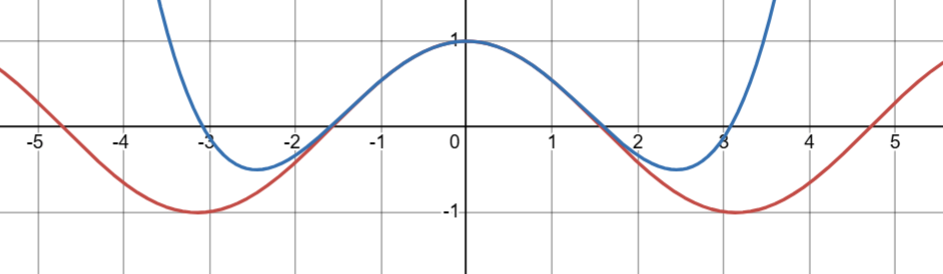
\includegraphics[width=0.5\textwidth]{images/taylorseries4.png}
\end{figure}

\subsection*{Improving approximations}
Finally, we should find a way to write a general rule for this polynomial. To do this, it is worth looking at how the derivatives are formed at each step:
\[p(x) = c_0 + c_1x + c_2x^2 + c_3x^3 + c_4x^4 + \dots\]
\[p'(x) = c_1 + 2\times c_2x + 3\times c_3x^2 + 4\times c_4x^3 + \dots\]
\[p''(x) = 2\times c_2 + 2\times 3\times c_3x + 3\times 4\times c_4x^2 + \dots\]
\[p^{(3)}(x) = 2\times 3\times c_3 + 2\times 3\times 4\times c_4x + \dots\]
\[p^{(4)}(x) = 2\times 3\times 4\times c_4 + \dots\]

Combining this with the derivatives of the function at each point:
\[f(0) = 1 = c_0 + c_1(0) + c_2(0)^2 + c_3(0)^3 + c_4(0)^4 + \dots \therefore c_0 = 1\]
\[f'(0) = 0 = c_1 + 2\times c_2(0) + 3\times c_3(0)^2 + 4\times c_4(0)^3 + \dots \therefore c_1 = 0\]
\[f''(0) = -1 = 2\times c_2 + (2\times 3)\times c_3(0) + (3\times 4)\times c_4(0)^2 + \dots \therefore c_2 = \frac{-1}{2}\]
\[f^{(3)}(0) = 0 = (2\times 3)\times c_3 + (2\times 3\times 4)\times c_4(0) + \dots \therefore c_3 = 0\]
\[f^{(4)}(0) = 1 = (2\times 3\times 4)\times c_4 + \dots \therefore c_4 = \frac{1}{2\times 3\times 4}\]

Hopefully you notice that the denominator of the $n^{th}$ term is $n$ factorial ($n!$).

This means that our polynomial could be:
\[p(x) = 1 - \frac{x^2}{2!} +\frac{x^4}{4!} - \frac{x^6}{6!} + \frac{x^8}{8!} - \dots\]

More specifically, we can write this as:
\[p(x) = \sum_{n=0}^{\infty} \frac{(-1)^{n}x^{2n}}{(2n)!}\]

\subsection*{Generalising the terms of a Taylor series}
You may have noticed that each term is calculated the same way, so we can generalise this.

If we consider the constant as the \textit{zero} term, the coefficient of the $n^{th}$ term can be found be taking the value of the $n^{th}$ derivative at the point we are forming the Taylor series about, and dividing it by $n!$.

In other words:
\[t_n = \frac{f^{(n)}(x)}{n!}\times x^n\]

Which means our Taylor series can be written as a sum:
\[p(x) = \sum_{n=0}^{\infty} \frac{f^{(n)}(x)}{n!}\times x^n\]

As an example, we can find the Taylor series for $f(x)=\ln{|2x+3|}$ about $x=0$:

First, find and evaluate the first few derivatives:
\[f'(x) = \frac{2}{2x+3}\]
\[f''(x) = -\frac{4}{(2x+3)^2}\]
\[f^{(3)}(x) = \frac{16}{(2x+3)^3}\]
\[f^{(4)}(x) = -\frac{96}{(2x+3)^4}\]
\[f^{(5)}(x) = \frac{768}{(2x+3)^5} \]

Using our generalisation and substituting in $x=0$, we can form the series:
\[f(x) = \ln{|2x+3|} = \ln{3} + \frac{2x}{3} - \frac{4x^2}{18} + \frac{16x^3}{162} - \frac{96x^4}{1944} + \frac{768x^5}{29160} - \dots\]

\begin{figure}[h]
    \centering
    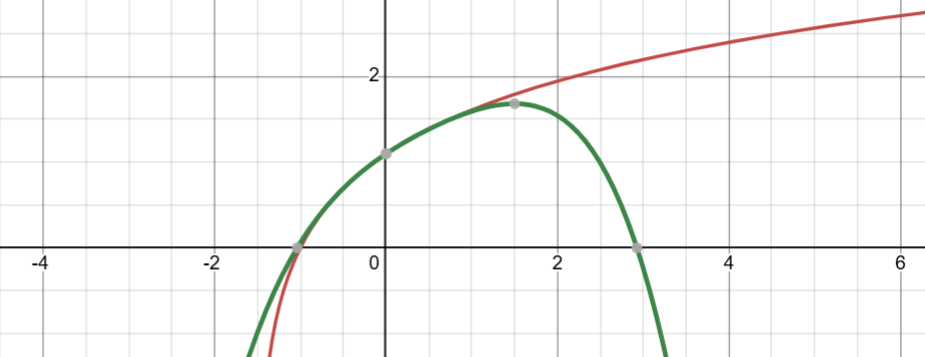
\includegraphics[width=0.5\textwidth]{images/taylorseries10.png}
\end{figure}

\pagebreak
\hypertarget{taylorserieslink}{\subsection*{Questions}}
\hyperlink{taylorseriesanswers}{(Answers - page {\pageref*{Taylor series answers}})}

\label{taylor series}
\begin{enumerate}[itemsep=1cm]
    \item 
    Derive the first two terms of the Taylor series to approximate the sine function about zero.

    \item 
    Derive the next two terms of this series, then generalise this as a sum.

    \item
    Derive the Taylor series for the function $f(x)=e^x$, finding the first six terms and generalising.

    \item
    Substitute $x=i\theta$ into the Taylor series for $e^x$ to show that $z=\cos{(\theta)}+i \sin{(\theta)}$ can also be written as $z=e^{i \theta}$.

    \item
    Find the Taylor series for the function $f(x) = 2x e^{-6x}$ about $x = 1$. Remember to use $x-1$ in the series, not just $x$.


\end{enumerate}
\end{document}